\subsection{Block Diagram}
\begin{figure}[h]
    \centering
    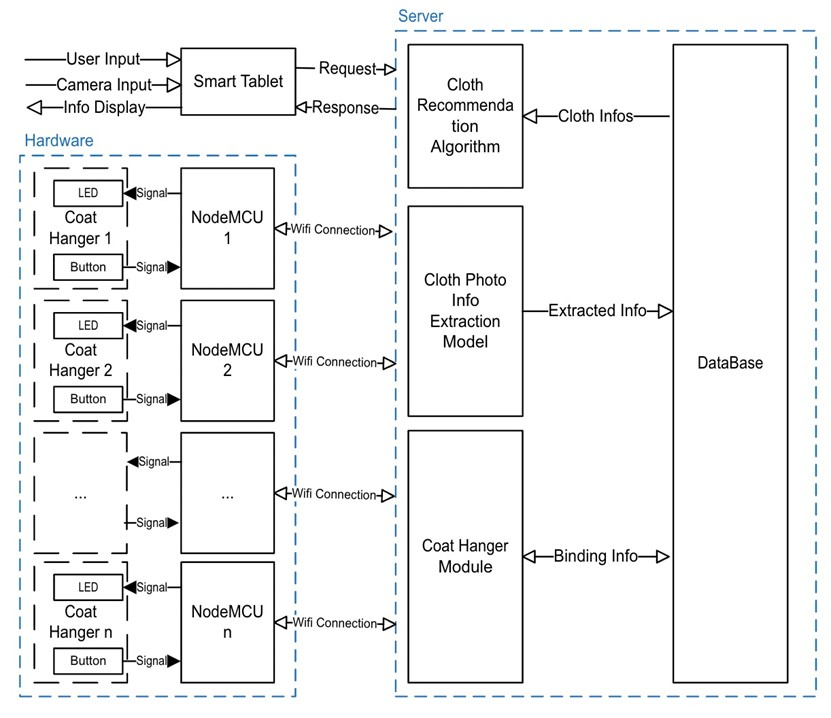
\includegraphics[width=12cm,height=12cm]{graph/block diagram.jpg}
    \caption{block diagram}
    \end{figure}

\subsection{Subsystem Overview}
\subsubsection{Coat Hanger}
\setlength{\parindent}{2em}This subsystem is in the form of coat hanger. When a pair of clothes is registered, a unique clothes ID is bound to the hanger ID and recorded in the database. After a certain pair of clothes is selected by the recommendation unit, the back-end server will broadcast ID information to the hanger through WIFI. The corresponding hanger needs to be activated and passes sound or light that indicates the location of the clothes.  

\noindent\textbf{Requirements}\quad This subsystem works as a hanger, should be strong, light and corrosion resistant. Different from those traditional hangers, we need to provide areas for the placement and certain protection of WIFI module, acousto-optic module and power supply module.    

\subsubsection{Clothes Photo Info Extraction Subsystem}
\setlength{\parindent}{2em}This subsystem serves as one of the core algorithms in our project, running in the back-end processor. The goal of this algorithm is to first achieve clothing parsing and segmentation to get bounding box and category information for each clothes detected from user’s registered clothes. The second task here is to predict clothes attribute such as floral, striped or knit. For each category of clothes, we will simply to several attributes. To build this algorithm, we will mainly use the mmfashion\cite{mmfashion}, which is a fashion analysis toolbox developed by Multimedia Lab, CUHK. 

\noindent\textbf{Requirements}\quad This subsystem should be able to detect and generate bounding box of each single pair of clothes, a relatedly high detection accuracy is required. The attributes need to be adapted to our application scenario. The overall detection and prediction time should be limited to a short period of time to prevent users from waiting too long.

\subsubsection{Outfit Recommendation Subsystem}
\setlength{\parindent}{2em}This subsystem serves as another core algorithm, takes clothes image, category and attribute as input. Some ConvNets will be tried for image encoding and GloVe for attribute encoding\cite{7890387}. We plan to Construct a three-dimensional graph structure, with similar (category, function etc.) clothes placed on the same layer, each node serves as one pair of clothes. A attributes-based distance function will be designed to determine the distance between each node. For the connectivity between different layer, we seek the advice of some fashion experts and establish rules, for example, evening dress and backpack are not suitable to use together. When generating an outfit, we use the idea of heuristic searching, for each layer we first find the several best matching items, then do the recommendation in the small group of graph structure. 

\noindent\textbf{Requirements}\quad This subsystem should be able to give high quality recommendation, which require us to give effective expert rules. For some of our potential customers, those who have too many clothes and need some advice on, the whole recommendation process should not take too long. Multiple recommendations need to be given to the user to choose from.

\subsubsection{Interactive Subsystem}
\setlength{\parindent}{2em}This subsystem is used for human-machine interaction. We will use Django for web and database control, A website will be designed for user accessing and database to store all the algorithm data and hanger-clothes pair information. Using our website, users can upload new clothes by taking photos, a virtual wardrobe feature helps users manage all their clothes, and an actionable display page of recommended clothes is for user to choose the one outfit to trace.

\noindent\textbf{Requirements}\quad This subsystem should be easy to use for our users. The database should be supported by the basic function of CRUD. Security considerations need to be taken care of, and user data should be kept properly. 

\subsubsection{NodeMCU Subsystem}
\setlength{\parindent}{2em}This subsystem is used for us to achieve the communication between our hangers and back-end server based on ESP8266 Wi-Fi MCU. We use MQTT as our communication protocol which designed for sensors or control devices with limited computing power and operating on low-bandwidth, unreliable networks. For each of our hanger, one MCU will be equipped, to communicate with our remote server for message acceptance (receiving the server's clothes trace request) and message sending (telling the server that the user has hung up his clothes).  

\noindent\textbf{Requirements}\quad This subsystem should be able to achieve the communicate between our server and hangers, the delay between them should not be too long and all messages send round trip should not miss their order or being dropped.

\subsection{Risk Analysis}  
\subsubsection{Failure of detecting attributes of the clothes accurately}
\noindent Failure of detecting attributes of the clothes accurately. Fashion attribute detection is not an easy problem in the area of computer vision. Therefore our detection accuracy might not be too high. To deal with this, we should carefully select the attributes we want to detect and could allow use to aid the system to make some decisions.
\subsubsection{Failure of the implementation of the hardware communication part}
\noindent Since we have no EE student in our team and have no experience with Node MCU chip and Wifi communication, we may encounter some issue during the implementation of this part. To deal with this, we need to start the implementation of the hardware part as soon as possible to avoid encountering some trouble at the last second.